\chapter{Methodology}
\label{ch:methodology}

Three systems are compared in this project: a rule-based heuristic baseline, T5-small used without any fine-tuning, and T5-small fine-tuned on the Cochrane-auto training pairs described in \cref{ch:data-preparation}. This chapter sets out how each was built.

\section{Rationale for Comparing Against Simple Baselines}
\label{sec:baseline-rationale}

A fine-tuned model is only interesting if it beats something simpler than itself. Including a hand-written baseline and an untrained version of the same architecture gives the fine-tuning result somewhere honest to stand against, rather than reporting a single number with nothing to compare it to.

\section{Heuristic Baseline}
\label{sec:heuristic-baseline}

The rule-based baseline was kept deliberately modest. Its purpose is not to compete seriously with a trained model but to show what plain rule-based editing can and cannot achieve on this kind of text, and to make sure any gain claimed for the transformer models is not simply matching what a few lines of regular expressions already produce.

It combines two operations. The first is a small, conservative substitution table that replaces around twenty common clinical and statistical terms with plainer equivalents, chosen because the replacement is close enough to synonymous in context that it does not risk changing the claim being made. \Cref{tab:lexicon-sample} shows a sample of these substitutions. The second operation splits sentences longer than 28 words at a safe boundary, such as a semicolon or a coordinating conjunction like ``however'' or ``although'', and leaves the sentence untouched if no safe split point is found rather than risking a broken sentence.

\begin{table}[htbp]
    \centering
    \caption{Sample of the lexical substitutions used in the heuristic baseline.}
    \label{tab:lexicon-sample}
    \begin{tabular}{@{}ll@{}}
        \toprule
        \textbf{Clinical term} & \textbf{Plain-language substitution} \\
        \midrule
        Participants & People \\
        Adverse events & Side effects \\
        Statistically significant & A real difference (unlikely due to chance) \\
        Confidence interval & Likely range of results \\
        Myocardial infarction & Heart attack \\
        Hypertension & High blood pressure \\
        Placebo & Dummy treatment \\
        \bottomrule
    \end{tabular}
\end{table}

One deliberate omission is worth stating directly. The baseline does not strip statistical detail held in parentheses, such as confidence intervals or effect sizes, even though removing it would make sentences look shorter and score better on surface readability formulas. Doing so would risk exactly the kind of meaning loss this project is designed to guard against, so the baseline was built to avoid that shortcut even at the cost of a slightly less impressive readability score.

\section{Zero-Shot Transformer Baseline}
\label{sec:zeroshot-baseline}

The second baseline is T5-small used exactly as published, with no fine-tuning on Cochrane-auto or any other simplification data. Inputs were given the standard text-to-text prefix \texttt{"simplify: "} followed by the source sentence, and outputs were generated with beam search (four beams, a maximum of 128 new tokens). This baseline isolates how much of any eventual improvement comes specifically from fine-tuning on domain data, rather than from the transformer architecture on its own.

\section{Fine-Tuning Procedure}
\label{sec:finetuning-procedure}

The main model is the same T5-small checkpoint, fine-tuned on the cleaned Cochrane-auto sentence pairs from \cref{ch:data-preparation}. \Cref{tab:hyperparameters} documents every setting used during training, in keeping with the reproducibility goals set out for this project.

\begin{table}[htbp]
    \centering
    \caption{Fine-tuning configuration for T5-small.}
    \label{tab:hyperparameters}
    \begin{tabular}{@{}ll@{}}
        \toprule
        \textbf{Setting} & \textbf{Value} \\
        \midrule
        Base model & \texttt{t5-small} (encoder-decoder, approx.\ 60M parameters) \\
        Task prefix & \texttt{"simplify: "} \\
        Maximum input length & 128 tokens \\
        Maximum target length & 128 tokens \\
        Training batch size & 4, with 2 gradient accumulation steps (effective batch size 8) \\
        Evaluation batch size & 4 \\
        Optimiser & AdamW, learning rate 3\,$\times$\,10\textsuperscript{-4}, weight decay 0.01 \\
        Early stopping & Patience of 2 evaluation epochs, monitoring validation loss \\
        Generation & Beam search, 4 beams, up to 128 new tokens \\
        \bottomrule
    \end{tabular}
\end{table}

The small per-device batch size and the use of gradient accumulation were dictated by the hardware available for this project, an Apple Silicon machine with 8GB of unified memory rather than a dedicated GPU with its own memory pool. Fine-tuning ran on the Metal Performance Shaders (MPS) backend, and gradient accumulation was used to reach an effective batch size of eight without exceeding the available memory during the backward pass.

The results reported in \cref{ch:results-discussion} come from a confirmation run using a training subset of 800 pairs over three epochs, intended to validate that the full pipeline, from data loading through to evaluation, behaves correctly end to end before committing to a longer run. \Cref{fig:training-loss} shows the training and validation loss recorded during this run. A full-scale run over the complete 7{,}075-pair training set for up to eight epochs, with the same early stopping criterion, is the natural next step once additional compute time is available, and \cref{ch:conclusion} returns to what that would be expected to change.

\begin{figure}[htbp]
    \centering
    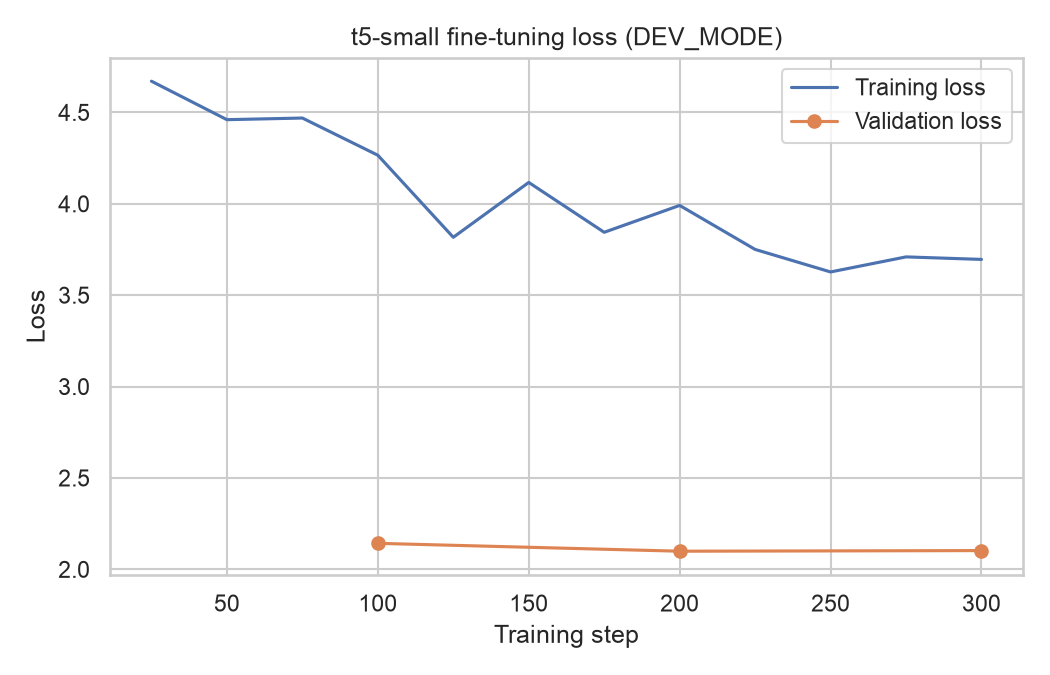
\includegraphics[width=0.8\textwidth]{figures/04_training_loss_curve.png}
    \caption{Training and validation loss during T5-small fine-tuning (confirmation run, 800 training pairs, three epochs).}
    \label{fig:training-loss}
\end{figure}
